\chapter{Compiling exceptions totally correctly}

\todo{Blah blah about differences between FP and total FP, substantiate the
title of the section}

The basic approach to compiling exceptions was shown in \cite{gmh:exceptions}.
This article provides excellent insight and inspiration how such code can be written
in a language such as Haskell.
However, peculiarities of programming with dependent types will make us
diverge a bit, in details at first, in parts of the design later.

\section{A simple exceptionless language}

All high-level languages in this thesis will be languages of simple, typed
expressions.

Our first language will feature only natural numbers and addition, not even
exceptions. We will implement it to build the auxiliary ecosystem of the
compiler and the skeleton of our development.

% branch: no-exceptions

\subsection{Type universe}


The first thing we will introduce is the type universe representing the set of
types of expressions of the high-level language. We will index our types with
values of this type (most notably the type \ident{Exp u} of expressions, to
indicate what the type of the expression is), and while we could use Agda types
directly for indexing, with an explicit universe, we get decidable equality of
types and all datatypes conveniently in \ident{Set}.

We could parametrize our
modules with the universe but let us just define a fixed one for the sake of
simplicity.

\begin{code}
  infixr 5 _=>\_
  data U : Set where
    nat : U
    _=>\_ : U -> U -> U
\end{code}

\todo{Omit the unused $\Rightarrow$ constructor entirely?}

\noindent We will also need the interpretation function \ident{el} that maps
types of our simple language to Agda types so that we can use Agda values in
the modelled language, talk about its denotational semantics etc.

\begin{code}
  el : U -> Set
  el nat = Nat
  el (s => t) = el s -> el t
\end{code}

\noindent And, as promised, equality is decidable on the elements of the
universe.

\begin{code}
  -- open import Relation.Nullary using (Dec)
  data Dec (p : Set) : Set where
    yes : p -> Dec p
    no  : ~ p -> Dec p

  -- open import Relation.Binary.PropositionalEquality using (_==\_)
  data _==\_ {a : Set} (x : a) : a -> Set where
    refl : x == x

  eqDecU : (u v : U) -> Dec (u == v)
  -- body omitted
\end{code}

\noindent We omit the body of \ident{eqDecU} because it's just an ordinary
uninteresting case analysis.

\note{In the following text, we will be a bit lax on wording related to type
universes.  We will be talking about ``expressions of the type \ident{u}'',
while actually referring to ``terms that represent expressions of \emph{the
type denoted by \ident{u}}''. This simplified approach can hardly cause
confusion, while adhering to precise wording in every situation at all costs
would lead to incomprehensible sentences.}

\subsection{Expressions}

The core of the language we are going to model consists of its expressions, of
course. For now, we will support nothing more than (numeric) literals and addition.
However, for further extensibility, we separate the type of binary operators.

The type of binary operators is indexed by the types of the two values that
the operator accepts as arguments; the third index represents the type of
the result of application of the operator on the two values.

\begin{code}
  data Op : U -> U -> U -> Set where
    Plus : Op nat nat nat
\end{code}

\noindent Now we can define the expressions: literals and binary operators.
Note that we index the datatype with elements of the universe \ident{U} so that
the Agda type of an expression also incorporates the type of the expression in
the modelled language.

\begin{code}
  data Exp : U -> Set where
    -- Literals
    Lit : forall {u} -> el u -> Exp u
    -- Binary operators
    Bin : forall {u v w} -> Bin u v w -> Exp u -> Exp v -> Exp w
\end{code}

\subsection{Semantics of expressions}

Our definition of the high-level language would not be complete without giving
the denotational semantics of its expressions. This is done in the following
pair of simple functions.

\begin{code}
  denOp : forall {u v w} -> Op u v w -> el u -> el v -> el w
  denOp Plus = _+\_

  denExp : forall {u} -> Exp u -> el u
  denExp (Lit x) = x
  denExp (Bin op l r) = denOp op (denExp l) (denExp r)
\end{code}

\noindent The separate type of binary operators deserves a separate function
converting an operator to a binary Agda function of the appropriate type.

Expressions are then turned into Agda values recursively; literals in a trivial
way, binary-operator expressions using the denotation of the corresponding
operator.

\subsection{Virtual machine}

We will use a very simple stack machine to run the compiled code.

\subsubsection{Stack}

The stack of
the machine is just a cons-list of values, indexed by types (elements of
\ident{U}) of the values pushed on the stack.  This means that just by looking
at the type of the stack, we can tell how many elements it contains and what
types they have.
\begin{code}
  -- open import Data.List
  infixr 5 _::_
  data List (a : Set) : Set where
    [] : List a
    _::_ : a -> List a -> List a

  Shape : Set
  Shape = List U

  infixr 5 _\scons\_
  data Stack : Shape -> Set where
    snil : Stack []
    _\scons\_ : forall {u s} -> el u -> Stack s -> Stack (u :: s)
\end{code}
\noindent The literal \ident{snil} represents the empty stack; new values are
pushed onto it using the infix constructor \ident{\bin{\scons}}.

\subsubsection{Instructions}

At this stage, the machine supports only two instructions: \ident{PUSH}
and \ident{ADD}.
\begin{code}
  data Instr : Shape -> Shape -> Set where
    PUSH : forall {u s} -> el u -> Instr s (u :: s)
    ADD : forall s -> Instr (nat :: nat :: s) (nat :: s)
\end{code}
The type of instructions is indexed by their action on stack. The first shape
argument is the required stack shape so that the instruction can be executed;
the second shape argument is the resulting shape of the stack after the
instruction has been executed.

For example, the instruction \ident{PUSH} takes any value of the type \ident{el u}
and pushes it onto a stack having any shape \ident{s}, creating a new
stack of the shape \ident{u :: s}.

The instruction \ident{ADD} represents popping two natural numbers from the
stack of any shape with two \ident{nat}s on top of it, (hence
\ident{nat :: nat :: s})
and subsequently pushing their sum onto it, resulting in the shape
\ident{nat :: s}.

\subsubsection{Code}

Finally, code for the stack machine is a sequence of instructions, where
type indices of subsequent instructions match. For example, if one instruction
in the sequence produces a stack of the shape \ident{nat :: nat :: s},
we want the next instruction in the code sequence to accept this shape.

If we regard
$\midt{Instr} : \midt{Shape} \to \midt{Shape} \to \midt{Set}$
as a binary relation on \ident{Shape}, then code is the \emph{transitive reflexive closure}
of \ident{Instr}, which is already included in the Agda standard library as the
module \ident{Data.Star}.

\begin{code}
  -- require import Data.Star
  infixr 5 _<|\_
  data Star {a b : Set} (R : a -> b -> Set) : a -> b -> Set where
    \nil : forall {x} -> Star R x x
    _<|\_ : forall {x y z} -> R x y -> Star R y z -> Star R x z
\end{code}

\begin{code}
  Code : Shape -> Shape -> Set
  Code = Star Instr
\end{code}

\noindent The type of instruction sequences is indexed in exactly the same
manner as the type of single instructions: the first index represents the
acceptable shape of stack before execution of the piece of code; the second
index represents the shape of stack after its execution.

Let us conclude this section with an utility function for concatenation of
instruction sequences, which is actually also included in \ident{Data.Star}.

\begin{code}
  infixr 5 _\app\_
  _\app\_ : forall {R x y z} -> Star R x y -> Star R y z -> Star R x z
  \nil \app ys = ys
  (x <| xs) \app ys = x <| xs \app ys
\end{code}

\subsection{Execution}

Now we will describe how the machine executes instructions, that is,
the operational semantics of the low-level language.

At this stage, the state of the machine is fully described by just its stack. This
means that there are no other state variables, registers or any additional
memory.

\subsubsection{Instructions}

Let us describe the effects of single instructions on the state of the machine
(that is, on the stack).

\begin{code}
  execInstr : forall {s t} -> Instr s t -> Stack s -> Stack t
  execInstr (PUSH x) st = x \scons st
  execInstr ADD (x \scons y \scons st) = (x + y) \scons st
\end{code}

\noindent The above function simply says that
\begin{itemize}
  \item the effect of the instruction \ident{PUSH} is pushing the attached
    value onto the stack. This consistently extends the information contained
    in the type of \ident{PUSH x}.\footnote{\ident{Instr s (u $::$ s)} -- for
    some \ident{u} and \ident{s}. This type is interpreted as ,,\ident{PUSH x}
    pushes some value of type \ident{u} onto the stack''.}
    What the type does not say (and \ident{execInstr}
    does) is what this value exactly is.
  \item the effect of the instruction \ident{ADD} pops two \ident{nat}s from
    the top of the stack and pushes their sum back.
\end{itemize}

Note that in this definition of the execution function, we already reap some
benefits of dependently typed programming.

First, of course, Agda checks types of the terms behind
the scenes and the machinery of types we have designed so far ensures that
in the case for \ident{PUSH x}, pushing the value \ident{x} always yields
a stack of the desired shape.

Second, in the case for \ident{ADD}, the types ensure that there are always two
\ident{nat}s on top of the stack and we can safely pattern-match with the
pattern \ident{x} \scons \ident{y} \scons \ident{st} -- because this match
will always succeed (and no other patterns for the \ident{ADD} case are needed). 

Thus the above definition complies to the type signatures involved (relatively
solid hints of correctness) and it is \emph{total} (esp. no pattern match failures),
while compilers of non-dependently typed languages, like OCaml or Haskell,
would complain about non-exhaustive patterns here --- there is no way to tell them
that, for example, we needn't deal with empty stacks when executing \ident{ADD}.

\todo{There's a paper saying that non-exhaustive matches are inevitable; insert
a reference.}

\subsubsection{Code}

Execution of code is then just a left fold over the sequence of instructions,
accepting the initial and yielding the resulting state of the machine.

\begin{code}
  execCode : forall {s t} -> Code s t -> Stack s -> Stack t
  execCode \nil st = st
  execCode (i <| is) st = execCode is (execInstr i st)
\end{code}

\noindent Execution of empty code has no effect on the stack; if the code
contains instructions, then the first instruction is executed and on the
resulting stack, the rest of code is executed.

\subsection{Compiler}

Compiling our simple high-level language for a stack machine is easy. The
central idea is that execution of an expression of some type is equivalent to
pushing its value onto the stack. Literal values are then pushed on the stack
directly; binary-operator expressions first evaluate both operands, effectively
putting their values on the top of the stack, and then execute the appropriate
instruction, determined by the operator. This instruction pops the top
two values from the stack as its operands and pushes the result back.

\begin{code}
  -- Syntactic sugar, promote an Instr to singleton Code
  [[_\;]] : forall {s t} -> Instr s t -> Code s t
  [[i\;]] = i <| \nil

  -- Determine what instruction performs the required calculation
  opInstr : forall {u v w} -> Op u v w -> forall {s} -> Instr (u :: v :: s) (w :: s)
  opInstr Plus = ADD

  -- Turn the expression into code
  compile : forall {u} -> Exp u -> forall {s} -> Code s (u :: s)
  compile (Lit x) = [[ PUSH x ]]
  compile (Bin op l r) = compile r \app compile l \app [[ opInstr op ]]
\end{code}

\noindent Again, behind the scenes, Agda ensures that all types match and the
code compiled by this function will not make the stack machine fail.\footnote{
  To be fair, this is already a property of \ident{Code}, ,,inherited'' by the
  function \ident{compile} via its return type.  However, it does constrain
possible definitions of the function \ident{compile}.} For example, there is no
way to have the function \ident{compile} output code where \ident{ADD} would
not have two \ident{nat}s on the top of the stack.

\subsection{Correctness}

This is the only place in this thesis where we will include the complete proof
of correctness. All proofs are of course contained in the attached Agda source
code.

\subsubsection{Operator lemma}

There are two auxiliary lemmas that we will need to prove our main result. The
first one of them is called \ident{op-correct} and it says that for any binary
operator, the instruction picked by the compiler indeed does what the
denotation of the binary operator says.

To be more specific, for any operator \ident{op} and two values \ident{x} and
\ident{y} of appropriate types, executing \ident{opInstr op} with the two
values on top of the stack results in having the value \ident{denOp op x y}
on the top of the stack afterwards.

\begin{code}
  op\-correct : forall {s u v w} {st : Stack s} {x : el u} {y : el w}
    -> (op : Op u v w)
    -> execInstr (opInstr op) (x \scons y \scons st) == denOp op x y \scons st
  op\-correct Plus = refl
\end{code}

\noindent In the case for \ident{Plus}, Agda substitutes the term \ident{Plus}
in the appropriate places, normalizes the resulting equality (expanding
function definitions etc.) and the proof becomes a trivial observation of
equality of normal forms, which is indicated by \ident{refl}.

\subsubsection{Distributivity lemma}

The other lemma that we will need says that execution of code distributes over
concatenation of code. In other words, executing the code \ident{c $\lhd\!\lhd$
d} has the same effect as first executing \ident{c} and then executing
\ident{d} on the resulting stack.

\begin{code}
  compile\-distr : forall {s t u} {st : Stack s}
    -> (c : Code s t) -> (d : Code t u)
    -> execCode (c \app d) st == execCode d (execCode c st)
\end{code}

\noindent We will proceed by induction on the parameter \ident{c}, which yields
two cases: either \ident{c} is empty or it consists of an instruction and the
rest of code. The first case is trivial by substituting $\varepsilon$ and
comparing the normal forms.

\begin{code}
  compile\-distr \nil d = refl
\end{code}

\noindent For writing the proof for the second case, we will use the wonderful
way supported by the Agda module $\midt{\equiv}$-\ident{Reasoning}\footnote{Actually,
there are also other similar modules, like \ident{$\le$-Reasoning} etc.}, which
lets us write proofs in the equational-reasoning style; just the way we would
do it with pen and paper.

\begin{code}
  compile\-distr (i <| is) d = begin
    execCode (i <| is \app d) st
      ==< refl \>
    execCode (is \app d) (execInstr i st)
      ==< compile\-distr is d \>
    execCode d (execCode is (execInstr i st))
      ==< refl \>
    execCode d (execCode c st)
    \qed
\end{code}

\noindent The proof begins with the word \ident{begin} and continues with the
first line, which is usually exactly the left-hand side of the equality we aim
to prove.  The second line contains the proof that the first line is equal to
the third line and so on -- by alternating terms and equality proofs, we can
gradually rewrite the left-hand term to the right-hand term of the desired
equality.

The first proof is just comparison of normal forms, as indicated by
\ident{refl}.

The second proof uses \ident{compile-distr} recursively as an induction
hypothesis to break the execution of composite code into two stages: first
executing \ident{is}, then executing \ident{d}.

The third proof is just \ident{refl} again and we use it to restructure the
term to the desired final form.

\subsubsection{Alternative proof of distributivity}

Starting from Agda 2.2.4, we can shorten our previous proof considerably
by using the \ident{rewrite} keyword:

\todo{Which version of Agda?}

\begin{code}
  compile\-distr : forall {s t u} {st : Stack s}
    -> (c : Code s t) -> (d : Code t u)
    -> execCode (c \app d) st == execCode d (execCode c st)
  compile\-distr \nil d = refl
  compile\-distr (i <| is) d rewrite compile\-distr is d (execInstr i st) = refl
\end{code}

\noindent The \ident{rewrite} construct expands to a specific pattern-matching
mechanism behind the scenes, effectively rewriting subterms of the goal using
the provided equality (which is the recursive application of
\ident{compile-distr} here). The resulting goal is then easily solvable by
\ident{refl}.

\subsubsection{Main correctness theorem}

This is the central result of this stage that relates together everything we
have defined so far in a single proof of correctness.

This proof formalizes the idea that we informally mentioned when we started to
write the compiler: executing the compiled code for an expression should be
equivalent to pushing the value of the expression (as given by the denotational
semantics) onto the stack.

\begin{code}
  correctness : forall {u s}
    -> (e : Exp u) (st : Stack s)
    -> execCode (compile e) st == denExp e \scons st
\end{code}

\noindent We will proceed by induction on the expression \ident{e}. The literal
case is trivial and solvable with \ident{refl}.

\begin{code}
  correctness (Lit x) _ = refl
\end{code}

\noindent The binary-operator case is a bit more involved and we will prove it
using equational reasoning, again.

\begin{code}
  correctness (Binop op l r) st = begin
    execCode (compile (Binop op l r)) st
      ==< refl \>
    execCode (compile r \app compile l \app [[ opInstr op ]]) st
      ==< compile\-distr (compile r) _ _ \>
    execCode (compile l \app [[ opInstr op ]]) (execCode (compile r) st)
      ==< compile\-distr (compile l) _ _ \>
    execCode [[ opInstr op ]] (execCode (compile l) (execCode (compile r) st))
      ==< cong (\lam z -> execCode [[ opInstr op ]] (execCode (compile l) z) (correctness r st) \>
    execCode [[ opInstr op ]] (execCode (compile l) (denExp r \scons st))
      ==< cong (\lam z -> execCode [[ opInstr op ]] z) (correctness l st) \>
    execCode [[ opInstr op ]] (denExp l \scons denExp r \scons st)
      ==< refl \>
    execInstr (opInstr op) (denExp l \scons denExp r \scons st)
      ==< op\-correct op \>
    denOp op (denExp l) (denExp r) \scons st
      ==< refl \>
    denExp (Binop op l r) \scons st
    \qed
\end{code}

\noindent The first \ident{refl} is used to expand the definition of compile
for the \ident{Binop} case so that human readers can see what's going on more
easily.

Then we make two appeals to the lemma \ident{compile-distr}. Each usage of this
lemma removes a part of the code sequence (exactly corresponding to an operand
of the binary operator) and transforms it to the effect that this piece of code
has on the stack until only a single instruction is left in the code sequence.
Note that we omit two of three arguments of \ident{compile-distr} in both
applications. This omission improves readability of the proof and Agda can
infer these terms, anyway.

The following two rather cryptic steps use the function \ident{cong} that allows
us to prove equality of two terms, given a proof of equality of their subterms
in a common context.

\begin{code}
  cong : forall {a b : Set} {x y : a}
    -> (f : a -> b)
    -> x == y -> f x == f y
\end{code}

\noindent This function is used with recursive applications of the theorem
\ident{correctness} to both operands of the binary operator. This allows us
to rewrite the subterms in the form \ident{execCode (compile operand) state}
to their equivalents in the form \ident{denExp operand \scons state}. These
two recursive applications are actually inductive hypotheses.

The two steps using \ident{exec-distr} and \ident{correctness} for each operand
actually correspond to ,,accelerated execution'' of these pieces of code -- we
do not execute the instructions; instead, we rely on the induction hypothesis
to simultaneously remove the code corresponding to the operand and push its
denotation onto the stack.

Finally, we use the lemma \ident{op-correct} to show that executing the
leftover instruction is exactly what is left to do to get the desired value
on top of the stack.

\subsection{Remarks}

Totality of Agda functions give us a proof of termination and the above
correctness proof gives us a guarantee that the compiler calculates the correct
code, given the defined semantics.

This is a very strong guarantee and it did not cost us that much -- the code we
have written looks much like the equivalent in any other functional language.
However, we have been maintaining much stronger invariants along the way, being
able to, for example, afford including only \emph{relevant}\footnote{In this
  context, by \emph{relevant} we mean the cases that arise during normal and
  expected operation of the program; for example, as already mentioned, we
needn't specify what to do when the instruction \ident{ADD} gets an
inappropriate number or types of elements on the stack -- just because this
cannot happen \emph{and the compiler knows it}.} pattern cases in a completely
safe way, without triggering compiler warnings.

Implementation-wise, the above (sub-)sections form separate modules in the
accompanying Agda code and these modules define the overall structure of our
development. In the following sections (and chapters), we will develop
the code further by extending and improving particular modules.

\section{Adding exceptions, GMH-style}

Now we are about to add exceptions to our language(s). The first approach is to
examine the ways found in the literature.

Code in this section is modelled after the paper \cite{gmh:exceptions} by
Graham Hutton and Joel Wright. The authors used Haskell in their development.
This approach was later formalized by Tobias Nipkow in \cite{nipkow} in
Isabelle, an interactive theorem prover/proof assistant, in exactly the same
way; the development even uses the same lemmas and their numbering as the
paper.

In contrast with the original paper and Tobias Nipkow's formalization thereof,
our aim is to create a dependently typed program, which means we don't want to
copy the Haskell code as is; instead, we will adapt it for the dependently
typed setting and see how it works out.

\subsection{Changes to the high-level language}

\subsubsection{Expressions}

The first module we need to extend when adding exceptions is the one containing
the definition of expressions of the high-level language. Namely, we need to
add the \ident{Throw} expression and the \ident{Catch} construct.

\begin{code}
  data Op : U -> U -> U -> Set where
    Plus : Op nat nat nat
\end{code}

\begin{code}
  data Exp : U -> Set where
    Lit : forall {u} -> el u -> Exp u
    Bin : forall {u v w} -> Op u v w -> Exp u -> Exp v -> Exp w
    Throw : forall {u} -> Exp u
    Catch : forall {u} -> (val : Exp u) -> (hnd : Exp u) -> Exp u
\end{code}

\noindent The type of expressions gets two new constructors.
\begin{itemize}

  \item One of them is \ident{Throw}, which is similar to the literal
    constructor \ident{Lit}, except that no value of the type \ident{el u} is
    needed: a throw-expression can promise to yield a value of any type without
    actually having it.

  \item The other one is \ident{Catch}. This constructor takes two expressions of
    the same type, the regular value and an exception handler, representing a
    catch-block.

\end{itemize}

\subsubsection{Semantics of expressions}

The expression type has just been extended with two new constructors and we
need to formalize what the meaning of the two expression variants actually is.
For that purpose, we need to alter the function \ident{denExp}.

The first change is in the return type of \ident{denExp}: we need a way to
indicate whether the expression evaluates to a value or whether an uncaught
exception occurs. To express that, the function \ident{denExp} will now return
\ident{Maybe (el u)} instead of the more direct \ident{el u}, using the value
\ident{nothing}\footnote{In contrast with Haskell, Agda uses lowercase initials
of the constructors \ident{just} and \ident{nothing}.} to indicate uncaught
exceptions and the value \ident{just x} to indicate that the expression
succesfully evaluates to the value~\ident{x}.

The second change is adding pattern cases for the newly added constructors
of \ident{Exp} to the denotation function \ident{denExp}.

\begin{code}
  denExp : forall {u} -> Exp u -> Maybe (el u)
  denExp (Lit x) = just x
  denExp (Bin op l r) with denExp l | denExp r
  \... | just x  | just y  = denOp op x y
  \... | just _  | nothing = nothing
  \... | nothing | just _  = nothing
  \... | nothing | nothing = nothing
  denExp Throw = nothing
  denExp (Catch e h) with denExp e
  \... | just x  = just x
  \... | nothing = denExp h 
\end{code}

\noindent We had to alter the original two cases slightly, most importantly the
binary operator case, where the result now yields a value (i.e.  doesn't throw)
if and only if both subexpressions yield values without throwing.

As hinted above, we added a case for the expression \ident{Throw}: this one
never yields a value and always throws; and also case for catch-expressions: if
no exception gets thrown in the value, the whole catch-expression is equivalent
to the regular value.  Otherwise, it is equivalent to the handler
value.\footnote{Especially, if both values throw exceptions, the
catch-expression propagates the exception thrown in the handler.}
\footnote{Hence, this constructor is similar to the combinator \ident{mplus} in
Haskell, which combines two possibly failing computations in exactly the same
way.}

\subsubsection{Remarks}

To keep things simple, the \ident{Throw} expression does not take a value,
unlike its counterparts in most programming languages. At this stage, we will
worry only about whether an exception has been thrown or not, not about its
particular value.

Also, in most programming languages, exception handlers can inspect the
exceptions being handled and return different values depending on some
attributes of the exception. In our language, it would be pointless to do that
because our exceptions do not carry values. Thus, our exception handlers are
just simple expressions of the same type as the main expression and they have
no means to refer to the exception being handled.

This concludes the definition of our high-level language and the rest of this thesis
will be mostly devoted to how to make it work operationally.

\subsection{Virtual machine}

What about our virtual stack machine and its low-level language of
instructions? What features and instructions do we need to add to make the
machine capable of computing with exceptions?

In \cite{gmh:exceptions}, Hutton and Wright give a description of how this can
be done. Let us extend the machine along the lines drawn by this paper and see
how we can adapt their solution to total functional programming with dependent
types, having the goals from the Introduction (page~\pageref{objectives}) in
mind.

\subsubsection{Stack}

First, Hutton and Wright propose altering the type of stacks because besides
values, now we are going to push exception handlers on the stack, too.

Unlike Hutton and Wright, we also need to care about stack shapes.
The type of stack shapes will no longer be a plain
list of types (that is, elements of the universe~\ident{U}); instead, we  will
distinguish between \emph{values} and \emph{handlers} pushed on the stack.
\footnote{Actually, there is even more ``dependent'' approach: we could
index the type of stack shapes by the list of handlers on the stack, getting
\ident{Shape : List U $\to$ Set}. In this setup, pushing a value on the stack
will change its shape but not the type of the shape, while pushing a handler
on the stack will change both the shape and the type of the shape. However, we
will not take this route as it turns out to be more complicated, while the author
could not see any advantages this would yield.}

\begin{code}
  data Item : Set where
    Val : U -> Item
    Han : U -> Item

  Shape : Set
  Shape = List Item
\end{code}
A value, denoted by \ident{Val u}, is an actual value of the type
denoted by \ident{u}; a handler, denoted by \ident{Han u}, is a piece of code
that, when run, leaves a value of the type \ident{u} on the top of the stack.
This naturally leads to the new type of stacks,
\begin{code}
  data Stack : Shape -> Set where
    snil : Stack []
    _\scons\_ : forall {u s} -> el u -> Stack s -> Stack (Val u :: s)
    _\sconsh\_ : forall {u s} -> Code s (Val u :: s) -> Stack s -> Stack (Han u :: s)
\end{code}
where the constructor \ident{\scons\!\!} corresponds to pushing values and the
constructor \ident{\sconsh\!\!} corresponds to pushing handlers on the stack.

Note that we push arbitrarily large strands of code as single items on the stack,
which contradicts one of our design principles -- that the
code must be executable on a simple stack machine (Introduction, page~\pageref{objectives})
-- and we will address this objection in \Fref{chap:compiling2}.

\subsubsection{Instructions and code}

Next, Hutton and Wright introduce three new instructions of the virtual machine:
\ident{MARK}, \ident{UNMARK}, and \ident{THROW}. In our code, this change
reflects in extending the \ident{Instr} type, which must now reside in a
\ident{mutual} block with \ident{Code}:

\begin{code}
  mutual
    data Instr : Shape -> Shape -> Set where
      PUSH : forall {u s} -> el u -> Instr s (Val u :: s)
      ADD : forall s -> Instr (Val nat :: Val nat :: s) (Val nat :: s)
      THROW : forall {u s} -> Instr s (Val u :: s)
      MARK : forall {u s} -> Code s (Val u :: s) -> Instr s (Han u :: s)
      UNMARK : forall {u s} -> Instr (Val u :: Han u :: s) (Val u :: s)

    Code : Shape -> Shape -> Set
    Code = Star Instr
\end{code}

\noindent The definition of code doesn't change: it is still a simple
``index-matching list'' of instructions.

\subsection{Execution, take one}

\subsubsection{Machine state}

The topic of machine state is left implicit in the paper by Hutton and Wright,
yet it is one of the most involved parts of this Agda development. We have to
make it completely explicit in order to adhere to our objectives.

To put it precisely, the state of the virtual machine includes
the following components:
\begin{itemize}
	\item the position in the executed code (``instruction pointer'');
	\item the stack;
	\item a bounded number of other flags and variables.
\end{itemize}

Then, execution is fully specified if for each instruction, we define its
effect on the machine state.

For now, we will leave the position in the code implicit and we will not count
it as a component of the state. The motivation for doing so is retaining
the ability to recurse over code structurally, which we would lose if we
permitted any manipulation with code (beyond un-consing done by the execution
function).

\subsubsection{Placeholder method}

One approach\footnote{This approach is not considered by Hutton and Wright at all;
we include it for illustration as the most na\"{i}ve strategy, whose disadvantages
will be gradually solved as we will be switching to better and better approaches.}
to execution not requiring any additional flags and variables
would be extending the stack type with a new constructor; let us call it
\ident{\void\scons\!\!\_}.
\begin{code}
  data Stack : Shape -> Set where
    snil : Stack []
    _\scons\_ : forall {u s} -> el u -> Stack s -> Stack (Val u :: s)
    _\sconsh\_ : forall {u s} -> Code s (Val u :: s) -> Stack s -> Stack (Han u :: s)
    \void\scons\_ : forall {u s} -> Stack s -> Stack (Val u :: s)
\end{code}
The new constructor acts as a placeholder for missing values if an exception is raised.

Note the strong similarity of the new constructor \ident{\void\scons\_} to the
\ident{THROW} instruction and the \ident{Throw}
expression. The instruction \ident{THROW} is indexed as an instruction that pushes
a value of any specified type on the stack -- but it actually does not. The 
\ident{Throw} expression is indexed as an expression that yields a value of any specified
type -- but it actually does not. Likewise, the \ident{\void} constructor is typed in
exactly the same way as the constructor that pushes values on the stack -- but it does not.

Thus, it is probably not a surprise that the \ident{THROW} instruction, instead of pushing
a value on the stack, pushes the \ident{\void} placeholder. To be precise, execution would
look the following way. \label{code:placeholder}
\begin{code}
  mutual
    execInstr : forall {s t} -> Instr s t -> Stack s -> Stack t
    -- the original two cases
    execInstr (PUSH x) st = x \scons st
    execInstr ADD (x \scons y \scons st) = (x + y) \scons st
    -- new instructions
    execInstr THROW st = \void\scons st
    execInstr (MARK h) st = h \sconsh st
    -- unmark: no exceptions thrown
    execInstr UNMARK (x \scons h \sconsh st) = x \scons st
    -- unmark: an exception thrown, handle it by executing the handler
    execInstr UNMARK (\void\scons h \sconsh st) = execCode h st
    -- miscellaneous exception handling
    execInstr ADD (\void\scons y \scons st) = \void\scons st
    execInstr ADD (x \scons \void\scons st) = \void\scons st
    execInstr ADD (\void\scons \void\scons st) = \void\scons st

    -- execCode is still a left fold over instructions
    execCode : forall {s t} -> Code s t -> Stack s -> Stack t
    execCode \nil st = st
    execCode (i <| is) st = execCode is (execInstr i st)
\end{code}

\noindent However, there are multiple downsides to this solution.

First, and most importantly, it's not really a transition to a different low-level language.
Instead, it is actually evaluation of the function \ident{denExp} with an explicit
stack. The placeholder \ident{\void} corresponds to the outcome \ident{nothing} of
\ident{denExp}, while the regular stack-cons using the constructor \ident{\scons\!\!}
corresponds to the outcome \ident{just x} (for some \ident{x}).

Second, this solution is not elegant in the sense that we need to add exception-handling
cases to every instruction (in our case, only \ident{ADD}). Why should we define how
these instructions handle exceptions when they all must do the same thing: just pass
the exception forward and do nothing else? Exceptions should be handled by a different
mechanism than regular execution.

Third, the Agda termination checker rejects the exception-handling case for
\ident{UNMARK} in the function \ident{execInstr}. Recursion isn't structural
here and we need to convince Agda about termination using a decreasing measure
or another way.

Fourth, it is not how machines actually work. Real exception-handling strategies do jumps,
and they don't push whole code blobs on the stack. Instead, they linearize exception-handling
code with regular code into a single instruction sequence -- and then jump to it if needed.

While this low-level representation does work, it leaves much to be desired. In the following
sections (and chapters), we will address these objections. Let us begin with the first two
of them.

\subsection{Execution, take two}

We will adapt the method of \emph{stack unwinding}, described in the paper by Hutton
and Wright. Now the machine will have two modes of execution, as hinted in
\cite[p.~7]{gmh:exceptions}.

The normal mode is exactly what one would expect: executing instructions on a stack, nothing surprising.

However, the non-trivial part is the exception-handling mode. When an exception is thrown,
two things need to be done in order to execute the exception handler: \label{subsubsec:stack-unwinding}
\begin{itemize}
	\item The stack needs to be unwound. This means removing items from the stack
		until the first exception handler.\footnote{Here we do not distinguish types
		of exception handlers so any handler is always appropriate. If we had typed
		exceptions, we might need to skip handlers that don't match the exception
		being processed.} When this is done, we can pop the handler from the stack
		and the resulting stack is now suitable for execution of the popped handler.
	\item The position in the sequence of instructions needs to be advanced
		appropriately. In general, we need to skip all instructions that belong
		to the computation being abandoned.
\end{itemize}

\subsubsection{Handler frames}
In a sense, we can talk about \emph{handler frames} that we need to discard
while looking for an exception handler. This is best demonstrated on an example.
Consider the following expression of the high-level language:
\begin{code}
  Bin Plus
  	(Catch
  		(Bin Plus (Lit 1) (Lit 4))
  		(Lit 2))
  	(Lit 3)
\end{code}
The above expression compiles to the following instruction sequence, where we use
the name~\ident{h} for the compiled handler code\footnote{In this case, the handler
code is \ident{[PUSH 2]}.} for readability.
\begin{code}
  [PUSH 3, MARK h, PUSH 4, PUSH 1, ADD, UNMARK, ADD]
\end{code}
This code does not throw any exceptions so we already know how it should be executed.
Let us plot the intermediate stacks in a graph, with the executed instructions
on the horizontal axis, and the stack growing vertically from the baseline. This is
how we get \Fref{fig:stack-frames}.

\begin{figure}[tp]
	\centering
	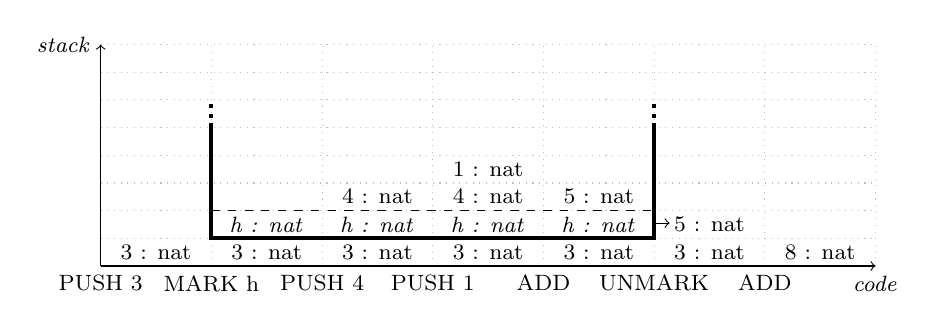
\begin{tikzpicture}[x=4em,y=1em,font=\footnotesize]
		\draw[lightgray,step=1,dotted] (0,0) grid (7,8);
		\draw[->] (0,0) -- (7,0) node[below] {\textit{code}};
		\draw[->] (0,0) -- (0,8) node[left] {\textit{stack}};

		\draw
			(0.5,0.5) node {\ident{3 : nat}}
			
			(1.5,0.5) node {\ident{3 : nat}}
			(1.5,1.5) node {\ident{\textit{h : nat}}}
			
			(2.5,0.5) node {\ident{3 : nat}}
			(2.5,1.5) node {\ident{\textit{h : nat}}}
			(2.5,2.5) node {\ident{4 : nat}}
			
			(3.5,0.5) node {\ident{3 : nat}}
			(3.5,1.5) node {\ident{\textit{h : nat}}}
			(3.5,2.5) node {\ident{4 : nat}}
			(3.5,3.5) node {\ident{1 : nat}}
			
			(4.5,0.5) node {\ident{3 : nat}}
			(4.5,1.5) node {\ident{\textit{h : nat}}}
			(4.5,2.5) node {\ident{5 : nat}}
			
			(5.5,0.5) node {\ident{3 : nat}}
			(5.5,1.5) node {\ident{5 : nat}}
			
			(6.5,0.5) node {\ident{8 : nat}}
			;
		\draw
			(0,0) node[below] {\ident{PUSH 3}}
			(1,0) node[below] {\ident{MARK h}}
			(2,0) node[below] {\ident{PUSH 4}}
			(3,0) node[below] {\ident{PUSH 1}}
			(4,0) node[below] {\ident{ADD}}
			(5,0) node[below] {\ident{UNMARK}}
			(6,0) node[below] {\ident{ADD}}
			;
		\draw[line width=1.5pt]
			(1,5) -- (1,1) -- (5,1) -- (5,5);
		\draw[line width=1.5pt,dotted]
			(1,5) -- (1,6)    (5,5) -- (5,6);
		\draw[dashed]
			(1,2) -- (5,2);
		\draw[->]
			(5,1.55) -- (5.14,1.55);
	\end{tikzpicture}
	\caption{Execution of an expression with the handler frame outlined.}
	\label{fig:stack-frames}
\end{figure}

The handler frame is delimited by the corresponding \ident{MARK} from the left,
the corresponding \ident{UNMARK} from the right, and the corresponding handler
on the stack from the bottom. Within the handler frame, evaluation of the
guarded\footnote{%
By ``guarded'' we mean that the expression is the main expression of
some catch-expression.
} expression runs independently from the context. Finally, after executing
\ident{UNMARK}, a single value is left on top of the stack: this is exactly
the denotation of the guarded expression.

Of course, handler frames may be nested since catch-expressions may also
be nested arbitrarily.
Hence, handler frames is what corresponds to catch-expressions on the operational
side of the matter.

\todo{Extended handler frames. Generalize for any expression. Exploitable for proving?
Is there some yet undiscovered direct 1:1 correspondence that would trivialize proofs?}

\subsubsection{Stack unwinding}
Now that handler frames are defined, we can describe exception handling
by stack unwinding quite concisely: abandon the innermost handler frame\footnote{%
Note that this involves discarding stack items but also skipping all instructions
that were to be executed within the handler frame.},
remembering the handler found at the bottom of the frame, and then
execute the handler as ordinary code on the resulting stack.

\subsubsection{Machine state}

As for the machine state, we discard our experiments with placeholders and return
to the original stack representation with two cons-constructors.
Instead of placeholders, we extend the state of the machine by distinguishing between
two modes of operation:
\begin{itemize}
	\item normal operation, where we just need to keep track of the stack;
	\item exception handling mode, where we keep additional state variables besides the stack.
\end{itemize}

\subsubsection{Differences to real machines}

In real machines, the above distinction would be represented by yet another
state variable determining which mode of operation the machine is in.
We will model it as different constructors of the \ident{State} data type.

Like in the placeholder method, we will push handlers on the stack, which
contradicts the principles we pursue and isn't really executable by real
machines. We will address this issue later, in Chapter \ref{chap:compiling2}.%
\footnote{This also causes trouble with termination but, unlike the
executability objection, termination issues can be worked around with
standard termination-proving methods or other tricks.}

For quitting the current handler frame, we need to skip all instructions
belonging to it. This is not so straightforward if we want to keep the
recursion structural. The termination checker of Agda requires that our
definitions be \emph{obviously} terminating, namely, structurally recursive,
which the following definition is not.
\begin{code}
  execCode : forall {s t} -> Code s t -> State s -> State t
  execCode nil state = state
  execCode (i <| is) state = execCode is (execInstr i state)
  execCode (THROW <| is) state = execInstr (skipToHandler is) state
\end{code}
In the snippet above, there is no single argument of \ident{execCode} that
obviously decreases in every recursive call: on the third line, the second
argument does not; on the fourth line, the first one does not -- and there
is no other argument that could possibly take the constantly-decreasing role.

There are several standard ways how to cope with this issue: accessibility
predicates, decreasing measures, or rewriting the algorithm to be
structurally recursive -- and we will aim for the last one.

This is the reason why we ``simulate'' the jump by switching the machine to an
alternative mode of execution and keep the function \ident{execCode}
structurally recursing over the instruction sequence.

Also, the type of the function \ident{execInstr}, that describes effects of
instructions on the machine state, takes only the instruction and state and
returns the new state. Since we don't include the ``instruction pointer'' in
the state, there is no way for the instructions to cause jumps in the code in
this setup without adding the special states or changing how execInstr works.

\todo{Not worse than GMH because they don't jump to addresses when looking for
the handler either; they even use implicit stacks.}

\subsubsection{Implementation}

The normal mode of operation contains simply the stack. However, the exceptional state
is a bit more involved; let us declare the datatypes and the auxiliary functions first
and describe them afterwards.

First, we need to know whether there is an appropriate handler on the stack and what type
it has. The shape of the stack is sufficient to determine this.
\begin{code}
  -- Get the type of the &\cident{n}&\-th top\-most handler in the Shape.
  -- Return &\cident{nothing}& if there is no such handler.
  unwindHnd : Shape -> \bN -> Maybe U
  unwindHnd (Han u :: xs) zero    = just u
  unwindHnd (Han _ :: xs) (suc n) = unwindHnd xs n
  unwindHnd (Val _ :: xs) n       = unwindHnd xs n
  unwindHnd []           _       = nothing
\end{code}

\noindent We also need to know what shape the unwound stack will have.
\begin{code}
  -- Unwind the shape up to just below the &\cident{n}&\-th top\-most handler.
  -- Return the empty shape if there is no such handler.
  unwindShape : Shape -> \bN -> Shape
  unwindShape (Han _ :: xs) zero    = xs
  unwindShape (Han _ :: xs) (suc n) = unwindShape xs n
  unwindShape (Val _ :: xs) n       = unwindShape xs n
  unwindShape []           _       = []
\end{code}

\noindent Now we can define the data types. First, the resumption point, which
represents information needed to resume computation after skipping the instructions
of the current handler frame.
\begin{code}
  -- Normal operation resumption point.
  data Resume (s : Shape) : Maybe U -> Set where
    -- A handler is available, also remember the stack on which
    -- the handler should operate.
    Caught : forall {u} -> Code s (Val u :: s) -> Stack s -> Resume s (just u)
    -- Uncaught throw.
    Uncaught : Resume s nothing
\end{code}

\noindent This finally allows us to define the data type of machine states, which represents
the two operational modes of the machine: normal mode and exception-handling mode.
\begin{code}
  data State : Shape -> Set where
  	-- Normal state
  	\tick[_] : forall {s} -> Stack s -> State s
  	-- Exception\-processing state
  	\x[_,_] : forall {s : Shape}
  	  -> (n : \bN&\!&)
  	  -> Resume (unwindShape s n) (unwindHnd s n)
  	  -> State s
\end{code}

\noindent As mentioned above, the alternative \ident{\tick[\_]} represents the normal mode
of operation, where the machine just needs to keep track of the stack.

The alternative \ident{$\times$[\_,\_]} represents the exception-handling state, described by
two (explicit) parameters.
\begin{itemize}
	\item The parameter~\ident{n} describes how many handler frames we need to
		\emph{unconditionally} unwind before starting to search for an exception handler.
		
		This is needed because while skipping instructions belonging to the current
		handler frame, we might enter additional handler frames nested within. Hence
		we need to keep track of the depth of nesting.
		
		This is exactly the point where Hutton \& Wright use an implied stack.\cite[pg.~7]{gmh:exceptions}
		In their function \ident{skip}, they use the implicit call stack to count
		the nesting levels. However, we want to make this counter explicit so we include
		it as a natural number into the machine state.
		
	\item The other parameter describes how to resume normal execution when
		the machine has finished skipping instructions.
		
		If there was an appropriate handler on the stack at the time of throwing
		the exception, this parameter contains the handler and the stack obtained
		by stack unwinding. If not, the (appropriately typed) constructor
		\ident{Uncaught} indicates that an uncaught exception was thrown.
\end{itemize}

\noindent Note that the whole machinery of types ensures a great part of correctness:
\begin{itemize}
	\item of course, types of all values, handlers and expressions match;
	\item resumption points representing uncaught exceptions cannot be included in the state
		if there is a handler on the stack;
	\item vice versa, resumption points representing handled exceptions cannot be included
		in the state if there is no handler on the stack.
\end{itemize}

Also note that in spite of these non-trivial data types used to model the
machine state, it is probably obvious that in real implementations, they boil
down to just a stack and a couple of additional state variables; with the
notable exception of an arbitrarily-sized handler in the case of the
constructor \ident{Caught}, which will be addressed later.

\subsubsection{Operation}

Now that we know what the state \emph{looks like}, we can take a look at how it \emph{works}.
This involves redefining the function \ident{execInstr} to describe effects of instructions
in our new setting.

But first, we need to define a prerequisite for \ident{execInstr}: the function
\ident{unwindStack} that calculates a resumption record from the given stack. This record
is needed for reinstation of computation once all appropriate instructions have been skipped.

\begin{code}
  unwindStack : forall {s} -> Stack s -> (n : \bN&\!&)
    -> Resume (unwindShape s n) (unwindHnd s n)
  unwindStack (h \sconsh xs) zero = Caught h xs
  unwindStack (h \sconsh xs) (suc n) = unwindStack xs n
  unwindStack (x \scons xs) n = unwindStack xs n
  unwindStack snil n = Uncaught
\end{code}

\noindent The function \ident{unwindStack}, in accord with the functions
defined above, takes a natural number \ident{n} denoting how many handler
frames are to be thrown right away before starting a search for a handler.  If
there are no suitable handlers, the alternative \ident{Uncaught} is returned.

Now we can proceed to the definition of the functions \ident{execInstr} and
\ident{execCode}, this time in a \ident{mutual} block.

\begin{codei}
  mutual
    execInstr : forall {s t} -> Instr s t -> State s -> State t
  	-- Normal operation
    execInstr ADD 			\tick[ x \scons y \scons st ]	= \tick[ (x + y) \scons st ]
    execInstr (PUSH x)		\tick[ st ] 		= \tick[ x \scons st ]
    execInstr (MARK h)		\tick[ st ] 		= \tick[ h \sconsh st ]
    execInstr UNMARK		\tick[ x \scons h \sconsh st ]	= \tick[ x \scons st ]
    -- Exception throwing  
    execInstr THROW			\tick[ st ] = \x[ zero , unwindStack st zero ] 
    -- Nontrivial exception processing
    execInstr (MARK _)		\x[ n	 ,	r	] = \x[ suc n, r ]
    execInstr UNMARK		\x[ suc n ,	r	] = \x[ n	, r ]
    execInstr UNMARK		\x[ zero	 , Caught h st	] = execCode h \tick[ st ]
    -- Trivial exception processing: instruction skipping
    execInstr THROW			\x[ n , r ] = \x[ n , r ]
    execInstr ADD			\x[ n , r ] = \x[ n , r ]
    execInstr (PUSH _)		\x[ n , r ] = \x[ n , r ]
\end{codei}
\begin{code}
    -- Code execution is still a left fold over instructions.
    execCode : forall {s t} -> Code s t -> State s -> State t
    execCode \nil st = st
    execCode (i <| is) st = execCode is (execInstr i st)
\end{code}

\noindent The above definition of the function \ident{execInstr} is mostly
straightforward.  First, we deal with the normal state, defining how it changes
when different instructions are executed.

The first block is essentially equivalent to what we defined for the
placeholder method (page~\pageref{code:placeholder}).

Then we define what effect the instruction \ident{THROW} has. The two actions
that constitute stack unwinding (page~\pageref{subsubsec:stack-unwinding}) are
represented as follows:

\begin{itemize}
	\item Popping items from the stack until a handler is found is done by the
		function \ident{unwindStack}. If a handler is found, it is returned
		along with the unwound stack as an instance of the constructor
		\ident{Caught}. Otherwise, an instance of the constructor
		\ident{Uncaught} is returned.
		The result of the function \ident{unwindStack} is then stored in the
		state of the machine.

	\item Skipping instructions that belong to the handler frame is done by
		switching the machine to the instruction-skipping state. The state also
		contains a natural number that keeps track of nesting depth of handler
		frames along the way (see the next paragraph for a more detailed
		description). This value is initially zero.
\end{itemize}

The reason why we need to keep track of the nesting depth is that instruction
skipping always ends at an \ident{UNMARK} instruction -- but not always the
first one encountered. The instruction sequence we want to skip may contain
more \ident{MARK}-\ident{UNMARK} pairs if the current handler frame contains
more nested handler frames. Hence we need to count \ident{MARK}s along the way
and then skip that number of \ident{UNMARK}s before stopping at the real
\ident{UNMARK} we are looking for.

Next, we define the core part of exception processing: dealing with the
instructions \ident{MARK} and \ident{UNMARK}.

In the exception-processing mode, the effect of the instruction \ident{MARK} is
quite trivial: it just increments the handler frame nesting counter contained
in the state.

If the frame nesting counter is nonzero, then the effect of the instruction
\ident{UNMARK} is trivial, too; it just \emph{decrements} the frame nesting
handler.

However, if the frame nesting counter is zero, the effect of the instruction
\ident{UNMARK} is a bit more complex: it can be described as switching the
machine to the normal mode using the saved stack, and then running the
saved exception handler.

This is exactly the point where we use the resumption record to reinstate
normal operation after having skipped all instructions that were to be skipped.

Note that in the non-trivial case for the instruction \ident{UNMARK}, we know
for sure that the state contains an instance of the \ident{Caught} constructor%
\footnote{As opposed to an instance of the \ident{Uncaught} constructor.}, so
we can be always sure there is a saved handler and stack available for
exception handling. The other option is simply ruled out by the type of the
stack: we are executing \ident{UNMARK}, whose type indicates that a handler
must be available.\footnote{To be explicit, because the type indices of the
	instruction \ident{UNMARK} and of the current state must match, the shape
	of the current state must contain a value \ident{Han u} for some \ident{u}
	as the second-to-top item.  This prevents the function \ident{unwindHnd}
from returning \ident{nothing}, but since \ident{nothing} is exactly the index
of \ident{Uncaught}, this constructor cannot occur in this situation.} This all
is understood by Agda and this pattern coverage is accepted as complete.

Finaly, we conclude our definition of the function \ident{execInstr} by
defining that in the exception-handling mode, all other instructions are not
interesting and they should be simply skipped without having any effect on the
machine state.

Note that, unlike in the placeholder method, there is only one case for each
such ``uninteresting'' instruction causing the machine to simply skip it, as
opposed to $2^{\mathrm{arity(instr)}} - 1$ cases in the placeholder method,
where we had to account for every possible combination of placeholders on the
stack. We have reduced both the number of cases, and their complexity.

Also note that in the whole specification, there are no implicit stacks: our
functions are completely tail-recursive. We designed the machine to work this
way to meet our requirements from the Introduction (page~\pageref{objectives}).

Both modes of execution are essentially the same; both contain stack, the
exception-handling mode also contains a number and a saved exception handler.
Thus only the arbitrarily-sized handler violates our simplicity requirement.
We will deal with this issue later in the Chapter \ref{chap:compiling2}.

\subsubsection{Termination}

However, this solution has a serious flaw: it is not structurally recursive.
As already mentioned, Agda will accept only definitions that are \emph{obviously}
terminating but the pair of functions \ident{execInstr} and \ident{execCode}
is not.

The apparent culprit is the call of \ident{execCode} from within
\ident{execInstr} in the non-trivial, exception-handling case for
\ident{UNMARK}. The function \ident{execCode} recurses structurally over its
first (explicit) argument, the code sequence. However, the handler that is to
be executed is not structurally smaller than the code sequence where the
\ident{UNMARK} came from, let alone \emph{obviously} structurally smaller.

\todo{Structurality not the only option. Measure. Bove-Capretta.}

\subsubsection{Correctness}

\todo{Proved in the attached Agda development.}


\begin{comment}
Then we have sex and see what effect it has on our placeholder..

... ... proceding...

Conclusion: sex has no effect on placeholder, but now i can finally think clearly...
thank you sex..
\todo{Trivial sex. processing / instructor skipping only.. only structural tail recursion}
\end{comment}





























































